% \VignetteIndexEntry{caret Manual -- Variable Importance}
% \VignetteDepends{caret}
% \VignettePackage{caret}
\documentclass[12pt]{article}
\usepackage{amsmath}
\usepackage[pdftex]{graphicx}
\usepackage{color}
\usepackage{xspace}
\usepackage{fancyvrb}
\usepackage{fancyhdr}
\usepackage{lastpage}
\usepackage{algorithm2e}
\usepackage[
         colorlinks=true,
         linkcolor=blue,
         citecolor=blue,
         urlcolor=blue]
         {hyperref}
         \usepackage{lscape}

\usepackage{Sweave}

%%%%%%%%%%%%%%%%%%%%%%%%%%%%%%%%%%%%%%%%%%%%%%%%%%%%%%%%%%%%%%%%%%

% define new colors for use
\definecolor{darkgreen}{rgb}{0,0.6,0}
\definecolor{darkred}{rgb}{0.6,0.0,0}
\definecolor{lightbrown}{rgb}{1,0.9,0.8}
\definecolor{brown}{rgb}{0.6,0.3,0.3}
\definecolor{darkblue}{rgb}{0,0,0.8}
\definecolor{darkmagenta}{rgb}{0.5,0,0.5}

%%%%%%%%%%%%%%%%%%%%%%%%%%%%%%%%%%%%%%%%%%%%%%%%%%%%%%%%%%%%%%%%%%

\newcommand{\bld}[1]{\mbox{\boldmath $#1$}}
\newcommand{\shell}[1]{\mbox{$#1$}}
\renewcommand{\vec}[1]{\mbox{\bf {#1}}}

\newcommand{\ReallySmallSpacing}{\renewcommand{\baselinestretch}{.6}\Large\normalsize}
\newcommand{\SmallSpacing}{\renewcommand{\baselinestretch}{1.1}\Large\normalsize}

\newcommand{\halfs}{\frac{1}{2}}

\setlength{\oddsidemargin}{-.25 truein}
\setlength{\evensidemargin}{0truein}
\setlength{\topmargin}{-0.2truein}
\setlength{\textwidth}{7 truein}
\setlength{\textheight}{8.5 truein}
\setlength{\parindent}{0.20truein}
\setlength{\parskip}{0.10truein}

%%%%%%%%%%%%%%%%%%%%%%%%%%%%%%%%%%%%%%%%%%%%%%%%%%%%%%%%%%%%%%%%%%
\pagestyle{fancy}
\lhead{}
\chead{Variable Importance Using The {\tt caret} Package}
\rhead{}
\lfoot{}
\cfoot{}
\rfoot{\thepage\ of \pageref{LastPage}}
\renewcommand{\headrulewidth}{1pt}
\renewcommand{\footrulewidth}{1pt}
%%%%%%%%%%%%%%%%%%%%%%%%%%%%%%%%%%%%%%%%%%%%%%%%%%%%%%%%%%%%%%%%%%

\title{ Variable Importance Using The {\tt caret} Package}
\author{Max Kuhn \\ max.kuhn@pfizer.com}


\begin{document}

\maketitle

\thispagestyle{empty}


\section{Variable Importance}

Variable importance evaluation functions can be separated into two groups: those that use the model information and those that do not. The advantage of using a model--based approach is that is more closely tied to the model performance and that it {\em may} be able to incorporate the correlation structure between the predictors into the importance calculation. Regardless of how the importance is calculated:
\begin{itemize}
\item For most classification models, each predictor will have a separate variable importance for each class (the exceptions are classification trees, bagged trees and boosted trees).
\item All measures of importance are scaled to have a maximum value of 100, unless the \texttt{scale} argument of \texttt{varImp.train} is set to \texttt{FALSE}.
\end{itemize}

\subsection{Model Specific Metrics}

The following methods for estimating the contribution of each
variable to the model are available
\begin{itemize}

   \item {\bf Linear Models:} the absolute value of the $t$--statistic
   for each model parameter is used.
   
   \item {\bf Random Forest:} from the R package: ``For
     each tree, the prediction accuracy on the out-of-bag portion of
     the data is recorded.  Then the same is done after permuting each
     predictor variable.  The difference between the two accuracies are
     then averaged over all trees, and normalized by the standard
     error.  For regression, the MSE is computed on the out-of-bag data
     for each tree, and then the same computed after permuting a
     variable.  The differences are averaged and normalized by the
     standard error.  If the standard error is equal to 0 for a
     variable, the division is not done.''
   
   \item {\bf Partial Least Squares}: the variable importance measure here is based on 
   weighted sums of the absolute regression coefficients. The weights are a function of
   the reduction of the sums of squares across the number of PLS components and are 
   computed separately for each outcome. Therefore, the contribution of the coefficients
  are weighted proportionally to the reduction in the sums of squares. 
  
   
  \item {\bf Recursive Partitioning}: The reduction in the loss function
  (e.g. mean squared error) attributed to each variable at each split is 
  tabulated and the sum is returned. Also, since there may be candidate variables
  that are important but are not used in a split, the top competing variables are
  also tabulated at each split. This can be turned off using the \texttt{maxcompete}
  argument in \texttt{rpart.control}. This method does not currently provide
  class--specific measures of importance when the response is a factor.
  
  \item {\bf Bagged Trees}: The same methodology as a single tree is applied to 
  all bootstrapped trees and the total importance is returned

  \item {\bf Boosted Trees}: This method uses the same approach as a single
  tree, but sums the importances over each boosting iteration (see the \texttt{gbm} package vignette).
  
  \item {\bf Multivariate Adaptive Regression Splines}: MARS models 
        include a backwards elimination feature selection routine that
        looks at reductions in the generalized cross-validation (GCV)
        estimate of error. The \texttt{varImp} function tracks the changes in
        model statistics, such as the GCV, for each predictor and
        accumulates the reduction in the statistic when each
        predictor's feature is added to the model. This total reduction
        is used as the variable importance measure. If a predictor was
        never used in any MARS basis function, it has an importance
        value of zero. There are three statistics that can be used to
        estimate variable importance in MARS models. Using
        \texttt{varImp(object, value = "gcv")} tracks the reduction in the
        generalized cross-validation statistic as terms are added.
        However, there are some cases when terms are retained 
        in the model that result in an increase in GCV. Negative variable 
        importance values for MARS are set to zero. Terms with non--zero importance that were not included
        in the final, pruned model are also listed as zero. 
        Alternatively, using
        \texttt{varImp(object, value = "rss")} monitors the change in the
        residual sums of squares (RSS) as terms are added, which will
        never be negative. 
        Also, the option \texttt{varImp(object, value = "nsubsets")} 
        returns the number of times that each variable is involved in a subset (in the final, pruned model).  
        Prior to June 2008, \texttt{varImp} used an internal function to estimate
        importance for MARS models. Currently, it is a wrapper around the 
       \texttt{evimp} function in the \texttt{earth} package.
   
  \item {\bf Nearest shrunken centroids}: The difference between the class
        centroids and the overall centroid is used to measure the
        variable influence (see \texttt{pamr.predict}). The larger the
        difference between   the class centroid and the overall center
        of the data, the larger the separation between the classes. The
        training set predictions must be supplied when an object of
        class \texttt{pamrtrained} is given to \texttt{varImp}. 

\end{itemize}   

\subsection{Model Independent Metrics}

If there is no model--specific way to estimate importance (or the argument \texttt{useModel = FALSE} is used in \texttt{varImp}) the importance of each predictor is evaluated individually using a ``filter'' approach. 

For classification, ROC curve analysis is conducted on each predictor. For two class problems, a series of cutoffs is applied to the predictor data to predict the class. The sensitivity and specificity are computed for each cutoff and the ROC curve is computed. The trapezoidal rule is used to compute the area under the ROC curve. This area is used as the measure of variable importance. For multi--class outcomes, the problem is decomposed into all pair--wise problems and the area under the curve is calculated for each class pair (i.e. class 1 vs. class 2, class 2 vs. class 3 etc.). For a specific class, the maximum area under the curve across the relevant pair--wise AUC's is used as the variable importance measure.

For regression, the relationship between each predictor and the outcome is evaluated. An argument, \texttt{nonpara}, is used to pick the model fitting technique. When \texttt{nonpara = FALSE}, a linear model is fit and the absolute value of the $t$--value for the slope of the predictor is used. Otherwise, a loess smoother is fit between the outcome and the predictor. The $R^2$ statistic is calculated for this model against the intercept only null model. This number is returned as a relative measure of variable importance.


\subsection{Example}

As an example, the multidrug resistance reversal (MDRR) agent data is used. First, we filter and standardize the predictors:

\begin{Schunk}
\begin{Sinput}
> options(width = 80)
> data(mdrr)
> set.seed(100)
> nzvColumns <- nearZeroVar(mdrrDescr)
> mdrrDescr <- mdrrDescr[, -nzvColumns]
> preProcVals <- apply(mdrrDescr, 2, processData)
> mdrrDescr <- applyProcessing(mdrrDescr, preProcVals)
\end{Sinput}
\end{Schunk}

Classification models were fit using random forests and partial least squares. The variable importance measures were calculated for these models and using the ROC method described above. 

\begin{Schunk}
\begin{Sinput}
> ctrl <- trainControl(verboseIter = FALSE)
> rfFit <- randomForest(mdrrDescr, mdrrClass, ntree = 2000, importance = TRUE)
> plsFit <- train(mdrrDescr, mdrrClass, "pls", tuneGrid = data.frame(.ncomp = 2 * 
+     (1:10)), trControl = ctrl)
> modelFree <- filterVarImp(mdrrDescr, mdrrClass)
> allImp1 <- data.frame(randomForest = varImp(rfFit)[, 1], PLS = varImp(plsFit$finalModel)[, 
+     1], ROC = modelFree[, 1])
> allImp1$note <- "All Descriptors"
\end{Sinput}
\end{Schunk}

A scatter plot matrices of the unscaled importances with a loess smooth curve are given in Figure \label{f:varImpSplom}. The top panel shows the results when the models use all predictors as inputs. Here, there is no 1:1 relationship between between methods. However, in the case of random forests, if a set of predictors are highly correlated, the selection of which predictor is used in a split is essentially random. This dilutes the importance of each of the correlated descriptors and may make the variable importance measures less helpful. 

To evaluate the effect of between--predictor correlations, descriptors with absolute pair--wise correlations above 0.90 are removed. In this case, the three methods show better agreement (the bottom panel of \label{f:varImpSplom}). 

\begin{Schunk}
\begin{Sinput}
> corrColumns <- findCorrelation(cor(mdrrDescr))
> mdrrDescr <- mdrrDescr[, -corrColumns]
> rfFit2 <- randomForest(mdrrDescr, mdrrClass, ntree = 2000, importance = TRUE)
> plsFit2 <- train(mdrrDescr, mdrrClass, "pls", tuneGrid = data.frame(.ncomp = 2 * 
+     (1:10)), trControl = ctrl)
> modelFree <- filterVarImp(mdrrDescr, mdrrClass)
> allImp2 <- data.frame(randomForest = varImp(rfFit2)[, 1], PLS = varImp(plsFit2$finalModel)[, 1], ROC = modelFree[, 1])
> allImp2$note <- "|Corr| < 0.90"
> allPred <- splom(~allImp1[, 1:3], type = c("p", "smooth"), main = "Variable Importance: All Predictors")
> filteredPred <- splom(~allImp2[, 1:3], type = c("p", "smooth"), main = "Variable Importance: |Corr| < 0.90 Filter")
\end{Sinput}
\end{Schunk}

Figure \ref{f:varImpInd} demonstrates the \texttt{plot} method for object of class \texttt{varImp}. In each case, needle plots are produced for the top predictors, based on their importance values. For classification models with more than 2 classes, the predictors are ordered by their average importance. With two classes, only one importance is plotted.

\begin{figure}[p]
   \begin{center}        
      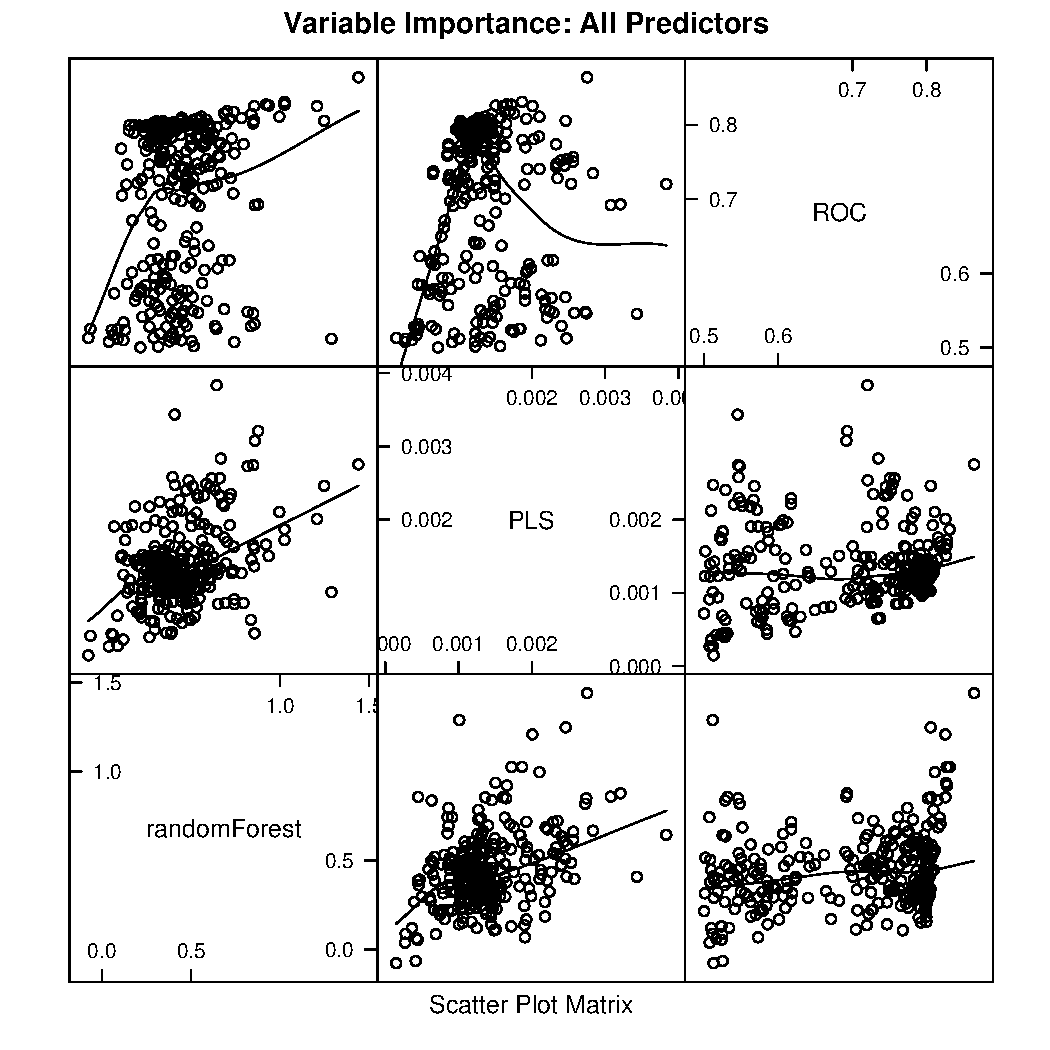
\includegraphics[clip, width = .5\textwidth]{allPred}
      
      \hspace*{.75 in}  
      
      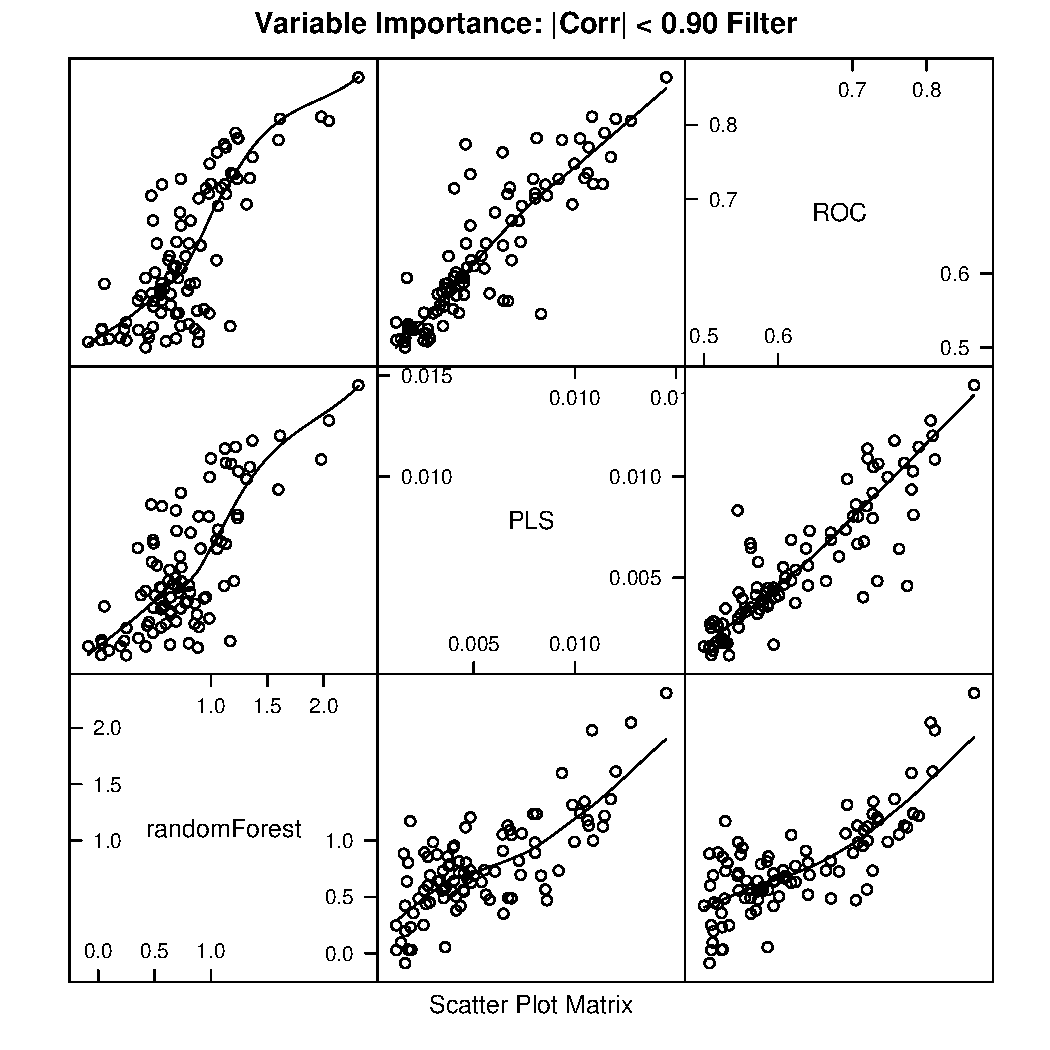
\includegraphics[clip, width = .5\textwidth]{filteredPred}     
      \caption{Relationships between different variable importance measures. The top panel shows a lack of linear correlation when all of the predictors are included in the model while the lower panel show the same techniques after a filter on between--predictor correlations.}
      \label{f:varImpSplom}         
   \end{center}
\end{figure}

\begin{figure}[hb]
   \begin{center}        
      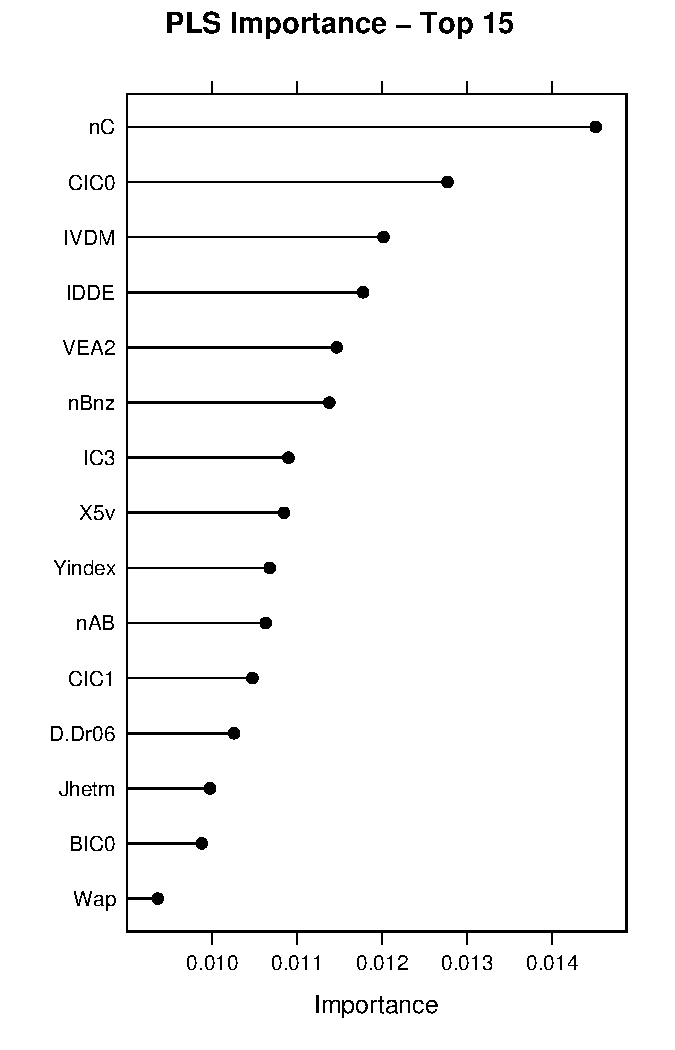
\includegraphics[clip, width = .45\textwidth]{plsVarImp}
      \hspace*{.5 in}  
      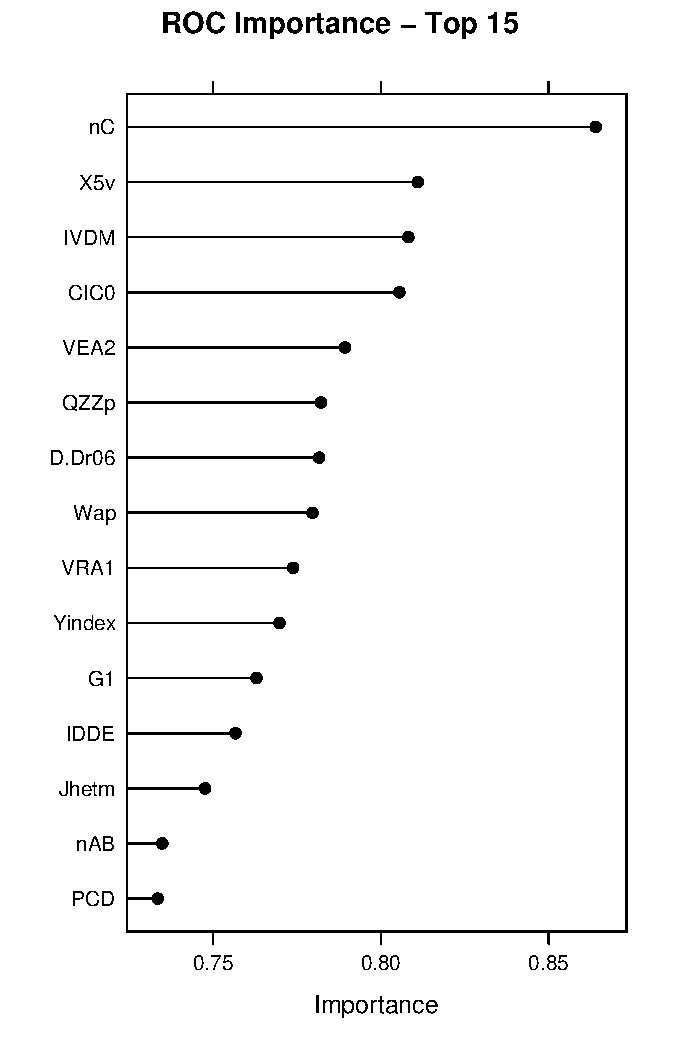
\includegraphics[clip, width = .45\textwidth]{rocVarImp}     
      \caption{Examples of two variable importance plots for the MBRR data. The left--hand panel is based on the partial least squares results and was generated using \texttt{plot(varImp(plsFit2), top = 15)}. The right--hand plot based on the univariate ROC curves and was generated using \texttt{plot(varImp(plsFit2, useModel = FALSE), top = 15)}. In each case, the unsupervised correlation filter was applied to the predictors prior to modeling}
      \label{f:varImpInd}         
   \end{center}
\end{figure}

\section{Session Information}

\begin{itemize}\raggedright
  \item R version 2.10.0 RC (2009-10-18 r50160), \verb|x86_64-apple-darwin9.8.0|
  \item Locale: \verb|en_US.UTF-8/en_US.UTF-8/C/C/en_US.UTF-8/en_US.UTF-8|
  \item Base packages: base, datasets, graphics, grDevices, grid,
    methods, splines, stats, tools, utils
  \item Other packages: akima~0.5-3, caret~4.36, class~7.3-1,
    e1071~1.5-20, earth~2.3-5, ellipse~0.3-5, gam~1.0.1, gbm~1.6-3,
    Hmisc~3.7-0, ipred~0.8-8, kernlab~0.9-9, klaR~0.6-0,
    lattice~0.17-26, leaps~2.9, MASS~7.3-3, mlbench~1.1-6, nnet~7.3-1,
    pls~2.1-0, plyr~0.1.9, proxy~0.4-4, randomForest~4.5-33,
    reshape~0.8.3, rpart~3.1-45, survival~2.35-7
  \item Loaded via a namespace (and not attached): cluster~1.12.1
\end{itemize}

\end{document}


